\documentclass{article}

\usepackage[margin=1in]{geometry}
\usepackage{tabularx}
\usepackage{amsmath}
\usepackage{tikz}
\usepackage{hyperref} % For clickable links

% Command for styling the boxes containing assignment instructions
\newcommand{\requirement}[1]{\noindent\fbox{\begin{minipage}{0.9\textwidth}
    \paragraph{Instructions}
    #1
\end{minipage} }}

\title{AI Powered Phishing Email Detection System}

\author{Mr. Rueben van der Westhuizen \\ u21434809}

\begin{document}

\maketitle

% Add project GitHub link to the front page
\begin{center}
\textbf{Project Repository:} \\[0.5em]
\href{https://github.com/21434809/AI-Powered-Phishing-Detection}{https://github.com/21434809/AI-Powered-Phishing-Detection}
\end{center}

\newpage
\tableofcontents
\newpage

\section{Research Overview}

\subsection{How does AI detect Phishing attacks:}

AI is increasingly used to detect phishing attacks by analyzing various email characteristics such as sender behavior, message content, and embedded URLs to identify anomalies or patterns indicative of phishing attempts \cite{basit2021comprehensive}. Machine learning algorithms, including natural language processing (NLP) and deep learning, are employed to recognize subtle cues that traditional rule  based systems might miss \cite{Wang2020Feature} \cite{Lauriola2021An}. ML algorithms, especially classifiers like Logistic Regression, Random Forests, and Neural Networks, are trained to identify patterns in email content, metadata, and even the tone of the language used can continuously learn from new data, improving their detection accuracy over time without manual updates \cite{Karim2019A} \cite{Murti2023Machine}.

\subsection{Traditional methods}

Compared to traditional methods, AI can handle large volumes of email traffic and detect novel, previously unseen phishing tactics. Its ability to adapt to new attack strategies makes it more effective in protection that is real time \cite{Jalil2022Highly} \cite{Alsariera2020AI} \cite{Basit2020A}.

\subsection{Advantages}
AI powered phishing detection is also less prone to false positives, ensuring legitimate emails are not mistakenly flagged. Additionally, AI systems can automate responses, reducing the need for manual intervention \cite{Basit2020A}. This leads to faster threat mitigation and enhanced user security \cite{Sameen2020PhishHaven—An}. By integrating AI, organizations can build a more robust defense against the evolving landscape of phishing threats \cite{Kumar2024What} \cite{Chinnasamy2024AI}.


\newpage

\section{Model selection process}
Selection of Kaggle's Phishing Email Dataset:
After close inspection, a combination off the "CEAS 08.csv" dataset, "NigerianFraud.csv", "SpamAssasin.csv", and "Nazario.csv" from has approximately 48,762 emails sum total after cleaning. 

\subsection{Data Preprocessing and Feature Extraction }

\begin{itemize}
    \item Subject: Has sufficient data without any missing values 
    \item Body: Has sufficient data without any missing values
    \item label (Spam or legitimate)
\end{itemize}


\subsection{Machine Learning Models Considered}
\begin{itemize}
    \item Logistic Regression
    \item Random Forest
    \item Neural Networks
\end{itemize}

\subsection{Model Selection Justification}
The model selection process for phishing email detection begins with evaluating the type of data available (email content, sender information, subject line, etc.) and the complexity of the task. Given that phishing emails often contain subtle cues, we need models that can identify these implied meaning in unstructured (text) data.

Initially, simpler models like Logistic Regression (LR) and Random Forest (RF) are considered. LR serves as a baseline because of its simplicity and interpretability, making it easier to understand which features are influencing the predictions. However, it may struggle with capturing nonlinear relationships and complex interactions between features.

On the other hand, Random Forest is an ensemble method that performs better on diverse datasets because it combines multiple decision trees, which helps in reducing overfitting. It is also able to capture nonlinear relationships in the data, making it more robust than LR.

For more complex patterns in the data, we consider Neural Networks (NN). Specifically, Multilayer Perceptrons (MLPs) or Recurrent Neural Networks (RNNs) are employed for text data, as they excel at recognizing sequential patterns in the email content, such as unusual phrasing or tone that might signal phishing. Additionally, long-short-term memory (LSTM) networks are considered for their ability to learn from sequences, making them highly effective for analyzing email texts with contextual meaning.

Model performance using metrics such as Accuracy, Precision, Recall, and F1-Score is crucial in evaluating phishing email detection systems. While Random Forest and Neural Networks typically offer the best results in terms of recall (catching phishing emails), Neural Networks—especially those with deep learning layers—tend to perform exceptionally well in detecting subtle, unseen phishing tactics. However, these models generally require longer training times, especially deep learning models, due to the complexity and the large amount of data they process during training.

Ultimately, Random Forest was selected for its balance between performance and interoperability and also provide feature importance scores.

\[
\begin{array}{|c|c|c|c|c|c|}
\hline
\textbf{Model} & \textbf{Accuracy (\%)} & \textbf{Precision (\%)} & \textbf{Recall (\%)} & \textbf{F1-Score (\%)} & \textbf{Notes} \\
\hline
\text{Logistic Regression} & 98.08 & 97.88 & 98.50 & 98.19 & \text{Simple, interpretable, fast} \\
\text{Random Forest} & 98.02 & 97.52 & 97.87 & 97.69 & \text{Handles non-linear data well} \\
\text{Neural Networks} & 99.40 & 98.70 & 99.00 & 98.80 & \text{Captures complex patterns} \\
\hline
\end{array}
\]
\newpage


\section{Requirements Specification}

The AI Powered Phishing Email Detection System is designed as a full stack web application that enables users to submit email content and receive real time predictions on whether the email is phishing or legitimate. The system leverages a machine learning backend and a user friendly frontend to provide accurate, fast, and interpretable results.

\subsection{Functional Requirements}
\begin{itemize}
    \item Users can submit email text (subject and body) via a web interface.
    \item The system processes the input and returns a prediction (phishing/legitimate) with a confidence score.
    \item The backend exposes a REST API endpoint for predictions.
    \item The frontend displays results, highlights suspicious words, and visualizes confidence.
    \item The system supports retraining and updating the ML model with new data.
\end{itemize}

\subsection{Non-Functional Requirements}
\begin{itemize}
    \item The system must respond to prediction requests within 2 seconds.
    \item The model must achieve at least 97\% accuracy on the test set.
    \item The web interface must be accessible and responsive on desktop and mobile devices.
    \item The backend and frontend must be easily deployable on standard Windows or Linux environments.
    \item Security: Only sanitized input is processed; no user data is stored.
\end{itemize}

\subsection{System Components}
\begin{itemize}
    \item \textbf{Frontend:} Angular SPA for user interaction.
    \item \textbf{Backend:} Flask REST API for ML inference.
    \item \textbf{ML Model:} Trained Random Forest, serialized as \texttt{model.pkl}.
    \item \textbf{Data:} Preprocessed datasets from multiple sources (CEAS, NigerianFraud, SpamAssassin, Nazario).
\end{itemize}
\newpage
\subsection{UML Diagrams} 
\begin{itemize}
    \item \textbf{System Architecture:} Shows the interaction between frontend, backend, and model.
    % Insert system architecture image
    \begin{figure}[h!]
        \centering
        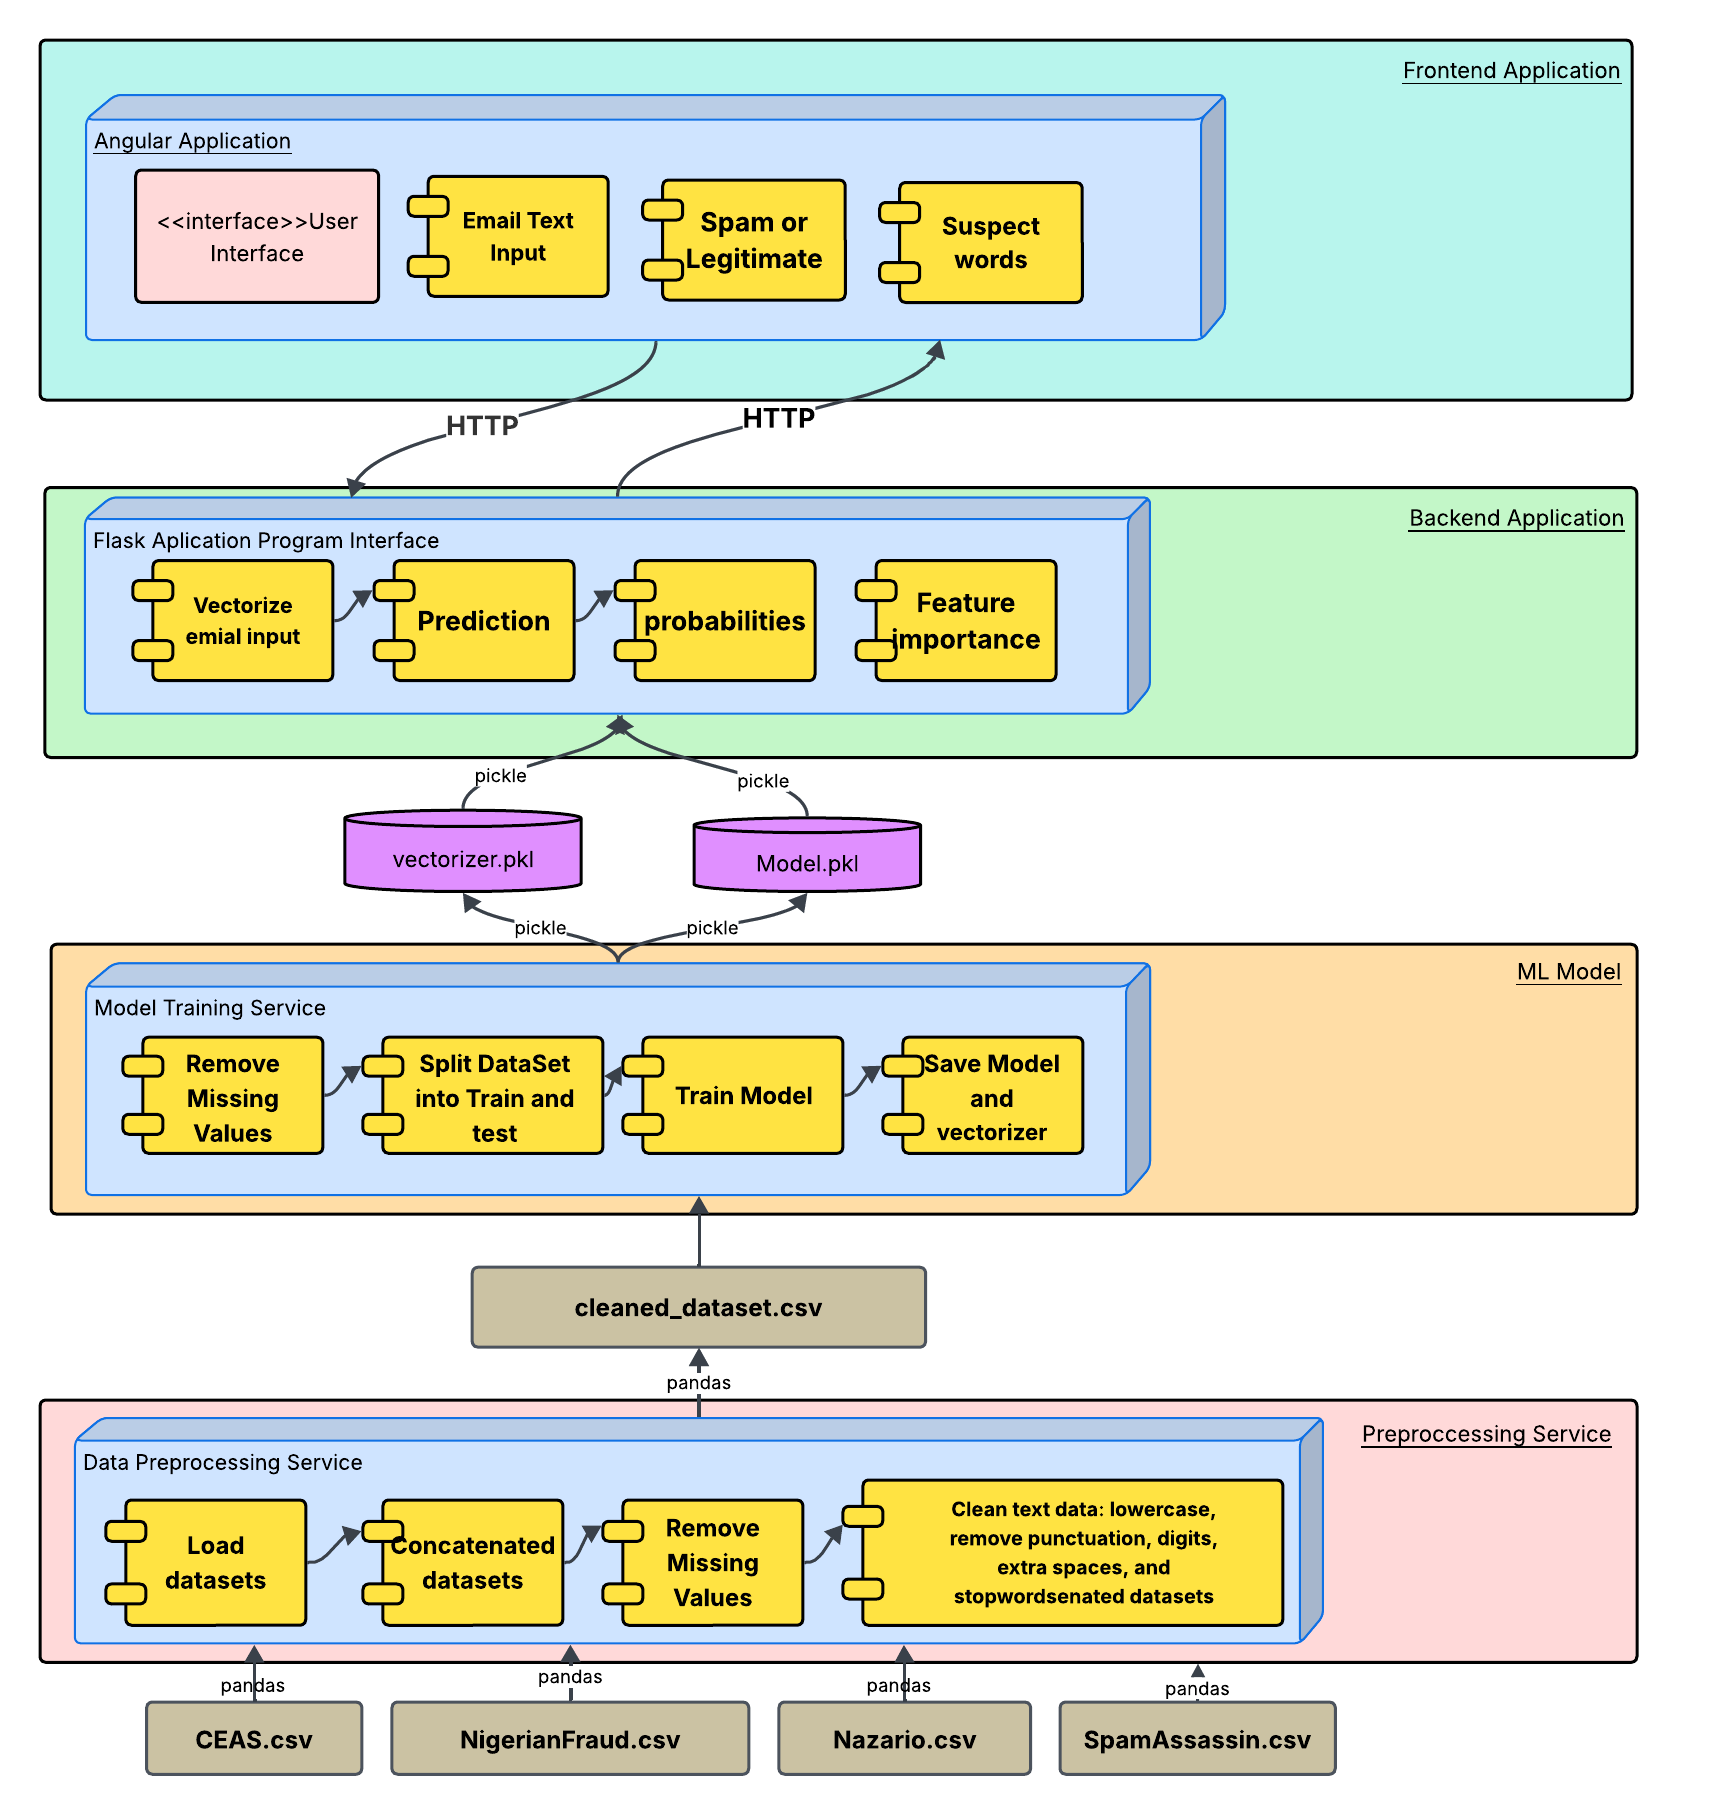
\includegraphics[width=0.8\textwidth]{Architecture.png}
        \caption{System Architecture of the AI Powered Phishing Email Detection System}
        \label{fig:system-architecture}
    \end{figure}

    \newpage
    \item \textbf{Workflow:} Sequence of user input, API call, prediction, and result display.
    % Insert system Sequence Diagrams image
    \begin{figure}[h!]
        \centering
        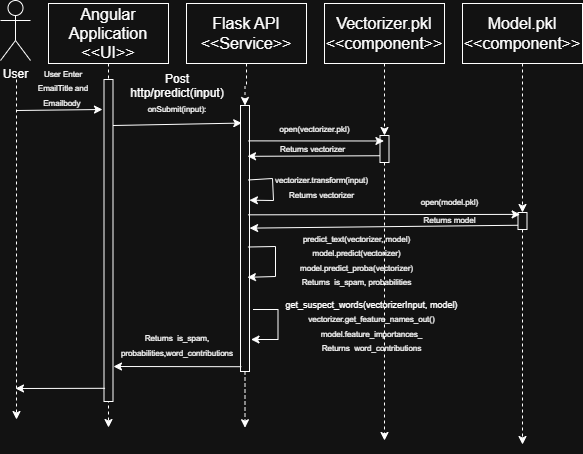
\includegraphics[width=0.8\textwidth]{Sequence.png}
        \caption{Workflow of the AI Powered Phishing Email Detection System}
        \label{fig:workflow}
    \end{figure}
    
\end{itemize}
\newpage
\section{Testing and Evaluation}

\subsection{Testing Methodology}
We conducted several tests to evaluate the prototype’s performance in realistic scenarios. Each test involved using either real or simulated emails to observe the system's behavior:
\begin{enumerate}
    \item \textbf{Known Phishing Example:}
    We used a known phishing email from the Gmail spam folder. The test performed well, with the model correctly identifying the email as phishing.
    \item \textbf{Legitimate Email Example:}
    We used a known legitimate email from the Gmail inbox. The test performed fairly, with the model correctly identifying the emails as legitimate. However, emails that follow a marketing template can be flagged as phishing, but with a low confidence score.
    \item \textbf{Curated Spear Phishing Email:}
    We used a curated spear phishing email based on a real legitimate email. The test performed fairly, with the model leaning more toward phishing, but with a low confidence score and a clear explanation of the words that were flagged as phishing.
    \item \textbf{Foreign Language Email:}
    We used a foreign language email based on a real legitimate email. The test performed poorly; it identified both legitimate and phishing emails as phishing, with a high confidence score and no clear explanation of the flagged words.
\end{enumerate}
\subsection{Evaluation Metrics}
We evaluated based on accuracy and and a classification report on 48,762 emails.
\begin{figure}[h!]
    \centering
    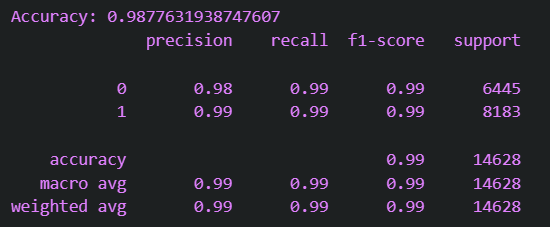
\includegraphics[width=0.8\textwidth]{classification_report.png}
    \caption{Classification Report of the AI Powered Phishing Email Detection System}
    \label{fig:classification-report}
\end{figure}
We also used confusion matrix to visualize the performance of the false positives and false negatives.
\begin{figure}[h!]
    \centering
    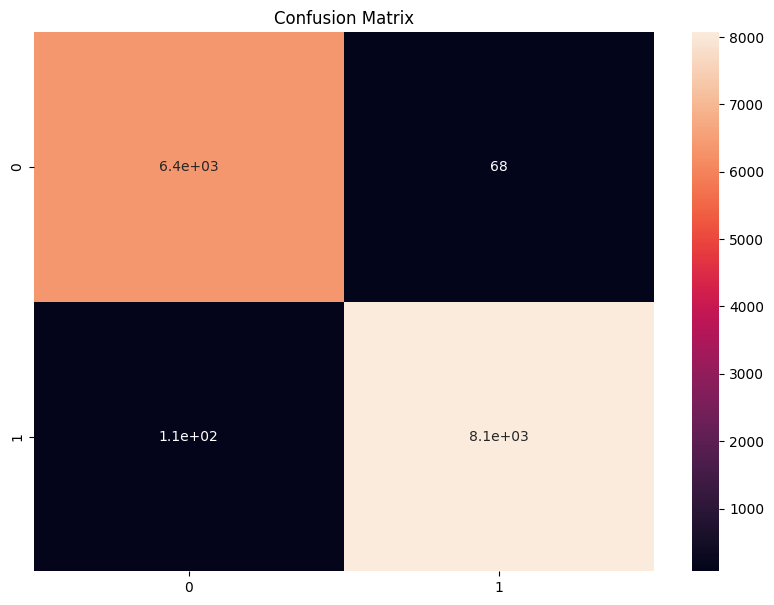
\includegraphics[width=0.4\textwidth]{confusion_matrix.png}
    \caption{Confusion Matrix of the AI Powered Phishing Email Detection System}
    \label{fig:confusion-matrix}
\end{figure}
In total there were only 111 false negatives and 68 false positives. The model is more likely to classify a legitimate email as phishing.
\newpage
\section{Conclusion}

\subsection{Summary of AI Principles}
The AI Powered Phishing Email Detection System leverages machine learning, specifically a Random Forest classifier, to distinguish between phishing and legitimate emails. The system uses natural language processing (NLP) techniques to extract features from the subject and body of emails. By training on a large, labeled dataset, the model learns to identify patterns and cues indicative of phishing attempts. The backend exposes a REST API for real-time inference, while the frontend provides an interactive interface for users to submit emails and receive predictions.

\subsection{Limitations}
Despite its strong performance, the system has several limitations:
\begin{itemize}
    \item \textbf{Dataset Bias:} The model is trained on public datasets that may not fully represent the diversity of real world emails, potentially reducing its effectiveness on novel or sophisticated phishing attacks.
    \item \textbf{False Positives:} Legitimate marketing emails and foreign language emails are sometimes misclassified as phishing, especially with high confidence, indicating limited generalization to non English or template based emails.
    \item \textbf{Limited Feature Set:} The model primarily uses the subject and body text, ignoring other useful features such as sender reputation, email headers, embedded URLs, and attachments.
    \item \textbf{Static Model:} The model does not learn continuously and requires manual retraining to adapt to new phishing tactics.
    \item \textbf{Language and Context:} The model struggles with non English emails and may not capture cultural or contextual nuances, leading to misclassification.
\end{itemize}

\subsection{Suggested Improvements}
To address these limitations, the following improvements are recommended:
\begin{itemize}
    \item \textbf{Expand and Diversify the Dataset:} Continuously collect and incorporate new, real-world phishing and legitimate emails, including multilingual and region-specific samples.
    \item \textbf{Feature Engineering:} Incorporate additional features such as sender domain analysis, URL reputation, attachment scanning, and email header inspection.
    \item \textbf{Continuous Learning:} Integrate user feedback with permission to retrain the model to adapt to new threats with minimal manual intervention.
\end{itemize}

\newpage

\bibliographystyle{bibstyle}
\bibliography{sources}

\end{document}
